\documentclass[a4paper,11pt,twoside]{article}
%\documentclass[a4paper,11pt,twoside,se]{article}

\usepackage{UmUStudentReport}
\usepackage{verbatim}   % Multi-line comments using \begin{comment}
\usepackage{courier}    % Nicer fonts are used. (not necessary)
\usepackage{pslatex}    % Also nicer fonts. (not necessary)
\usepackage[pdftex]{graphicx}   % allows including pdf figures
\usepackage{listings}
\usepackage{pgf-umlcd}
%\usepackage{lmodern}   % Optional fonts. (not necessary)
%\usepackage{tabularx}
%\usepackage{microtype} % Provides some typographic improvements over default settings
%\usepackage{placeins}  % For aligning images with \FloatBarrier
%\usepackage{booktabs}  % For nice-looking tables
%\usepackage{titlesec}  % More granular control of sections.

% DOCUMENT INFO
% =============
\department{Department of Computing Science}
\coursename{Object-Oriented Programming Methodology 7.5 p}
\coursecode{5DV133}
\title{OU1 Clock}
\author{Lorenz Gerber ({\tt{dv15lgr@cs.umu.se}} {\tt{lozger03@student.umu.se}})}
\date{2016-04-07}
%\revisiondate{2016-01-18}
\instructor{Anders Broberg / Niklas Fries / Adam Dahlgren / Jonathan
  Westin / Erik Moström / Alexander Sutherland}


% DOCUMENT SETTINGS
% =================
\bibliographystyle{plain}
%\bibliographystyle{ieee}
\pagestyle{fancy}
\raggedbottom
\setcounter{secnumdepth}{2}
\setcounter{tocdepth}{2}
%\graphicspath{{images/}}   %Path for images

\usepackage{float}
\floatstyle{ruled}
\newfloat{listing}{thp}{lop}
\floatname{listing}{Listing}



% DEFINES
% =======
%\newcommand{\mycommand}{<latex code>}

% DOCUMENT
% ========
\begin{document}
\lstset{language=C}
\maketitle
\thispagestyle{empty}
\newpage
\tableofcontents
\thispagestyle{empty}
\newpage

\clearpage
\pagenumbering{arabic}

\section{Introduction} 


\section{Usage Instructions}
which files included, how to compile, how to run from shell with javac
and java, in and out data of the program.

\section{System Description}
class diagram, Class Responsibility and Collaborators, programflow

\section{Unit Testing}




\begin{figure}
  \centering
  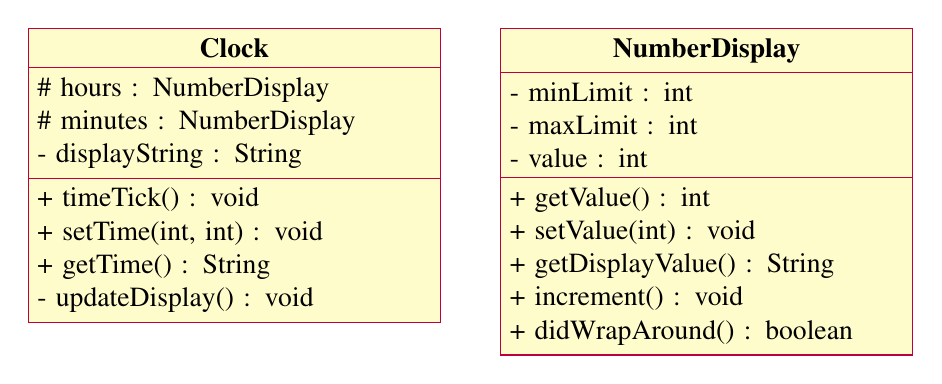
\begin{tikzpicture}
    \begin{class}[text width = 5cm]{Clock}{0,0}
      \attribute{\# hours : NumberDisplay}
      \attribute{\# minutes : NumberDisplay}
      \attribute{- displayString : String}

      \operation{+ timeTick() : void}
      \operation{+ setTime(int, int) : void} 
      \operation{+ getTime() : String}
      \operation{- updateDisplay() : void}
    \end{class}

    \begin{class}[text width = 5cm]{NumberDisplay}{6, 0}
      \attribute{- minLimit : int}
      \attribute{- maxLimit : int}
      \attribute{- value : int}

      \operation{+ getValue() : int}
      \operation{+ setValue(int) : void}
      \operation{+ getDisplayValue() : String}
      \operation{+ increment() : void}
      \operation{+ didWrapAround() : boolean}
    \end{class}
  \end{tikzpicture}
  \caption{\textit{Class diagrams of Clock and NumberDisplay.}}
  \label{fig:umlclass}  
\end{figure}


\section{Program Structure}

\section{Discussion}



\addcontentsline{toc}{section}{\refname}
\bibliography{references}

\end{document}
